\section{Graph theory}

Numerous decision-making problems find their representation in the realm of graphs.
\begin{definition}[\textit{Graph}]
    A graph is described as a pair $G=(N,E)$, comprising a set of nodes denoted as $N$ and a set of edges or arcs $E$, where these edges link the nodes in pairs.
\end{definition}   
\begin{definition}[\textit{Directed and undirected graphs}]
    In the case of an undirected graph, an edge connecting nodes $i$ and $j$ is denoted as ${i,j}$, while in a directed graph, it is represented as $(i,j)$.    
\end{definition}
\begin{example}
    Consider a road network connecting a total of "n" cities, which can be effectively represented by a graph. 
    In this representation, each city corresponds to a node, and the connections between them are represented as edges.        
    \begin{figure}[H]
        \centering
        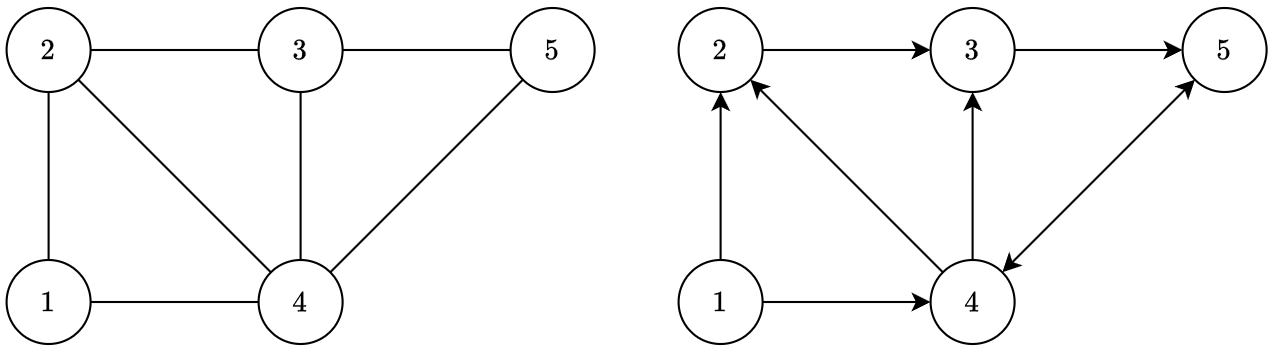
\includegraphics[width=0.6\linewidth]{images/graph.png}
    \end{figure}
    The left graph is undirected and defined as follows:
    \begin{itemize}
        \item $N=\{1,2,3,4,5\}$
        \item $E=\{\{1,2\},\{1,4\},\{2,3\},\{2,4\},\{3,4\},\{3,5\},\{4,5\}\}$
    \end{itemize}
    The right graph is directed and defined as:
    \begin{itemize}
        \item $N=\{1,2,3,4,5\}$
        \item $E^{'}=\{(1,2),(1,4),(2,3),(2,4),(3,4),(3,5),(4,5)\}$
    \end{itemize}
\end{example}
\newpage
\begin{definition}[\textit{Adjacent node}]
    Nodes are considered adjacent when they are linked by an edge.
\end{definition}
\begin{definition}[\textit{Incident edge}]
    An edge labeled as $e$ is deemed incident to a node $v$ when node $v$ serves as one of the endpoints of the edge $e$.
\end{definition}
\begin{definition}[\textit{Degree of a node}]   
    In undirected graphs, the degree of a node signifies the count of edges incident to that particular node. 
\end{definition}
\begin{definition}[\textit{In-degree and out-degree of a node}]   
    In directed graphs, the in-degree of a node represents the number of arcs that have it as their successor, while the out-degree of a node denotes the quantity of arcs that have it as their predecessor.
\end{definition}
\begin{example}
    In the undirected graph, we observe that nodes 1 and 2 are adjacent, while node 1 and node 3 are not. 
    The edge $\{1,2\}$ is incident to nodes 1 and 2. 
    Node 1 has a degree of 2, and node 4 has a degree of 4.
    In the directed graph, node 1 exhibits an in-degree of 0 and an out-degree of 2.
    \begin{figure}[H]
        \centering
        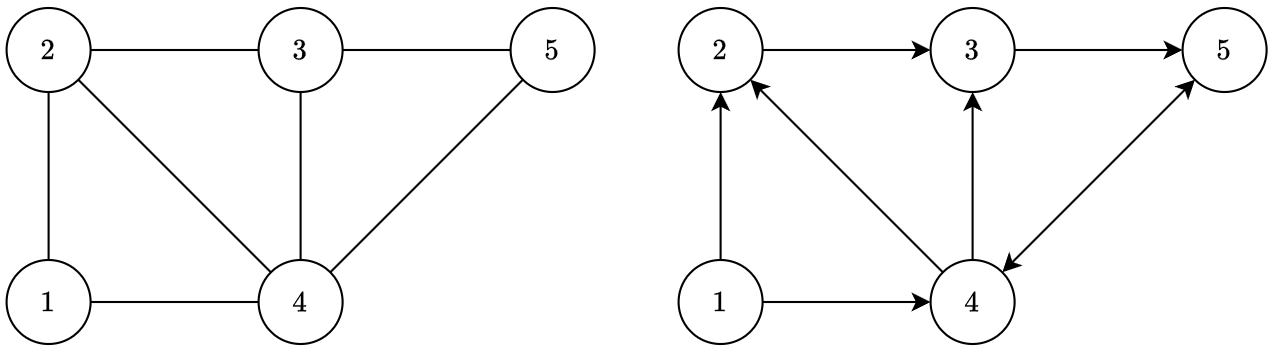
\includegraphics[width=0.6\linewidth]{images/graph.png}
    \end{figure}
\end{example}
\begin{definition}[\textit{Directed path}]
    A directed path from $i \in N$ to $j \in N$ is a sequence $p=\langle \{v_1,v_2\},\{v_2,v_3\},\dots,\{v_{k-1},v_k\}\rangle $ connecting nodes $v_1$ and $v_k$.
\end{definition}
\begin{definition}[\textit{Connected nodes}]   
    Nodes $u$ and $v$ are connected if there is a path connecting them. 
    A graph $(N,E)$ is connected if $u,v$ are connected for any $u,v \in N$. 
\end{definition}
\begin{definition}[\textit{Strongly connected nodes}]      
    A graph is \emph{strongly connected} if $u$ and $v$ are connected by a directed path for any $u,v \in N$. 
\end{definition}
\begin{definition}[\textit{Cycle}]      
    A cycle or circuit is a path with $v_1=v_k$.
\end{definition}
\begin{example}
    The undirected graph has a path $\langle \{2,3\},\{3,4\},\{4,5\}\rangle$ connecting node $2$ to node $5$, thus indicating a connection between these nodes.
    
    The directed graph has a directed path $\langle (3,5),(5,4),(4,2),(2,3),(3,4) \rangle$ from node $3$ to node $4$. So we say those nodes are not strongly connected. 
    
    In the undirected graph, we observe a cycle $\langle \{2,3\},\{3,5\},\{5,4\},\{4,2\}\rangle$. 
    In the directed graph, a circuit is present, specifically $\langle (2,3),(3,4),(4,2) \rangle$. 
    \begin{figure}[H]
        \centering
        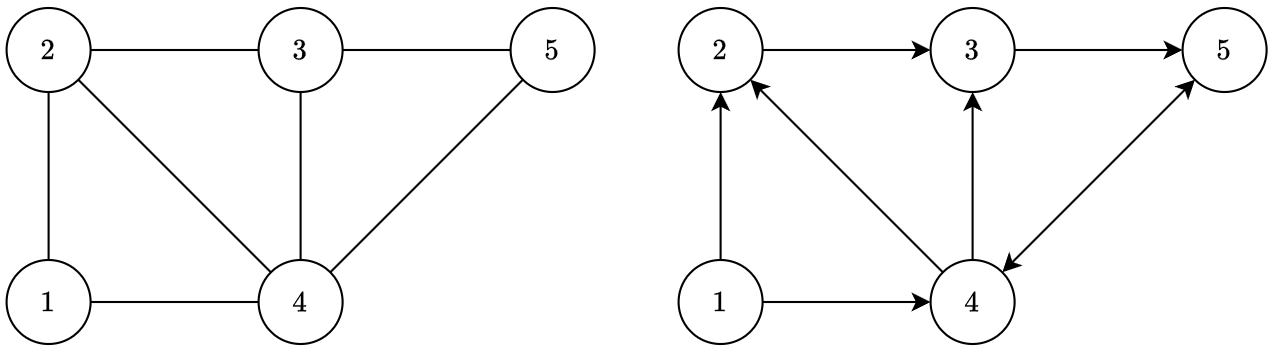
\includegraphics[width=0.6\linewidth]{images/graph.png}
    \end{figure}
\end{example}
\newpage
\begin{definition}[\textit{Bipartite graph}]
    A graph is bipartite if there is a partition $N=N_1 \cup N_2$ with $N_1 \cap N_1 = \varnothing$ such that no edge connects nodes in the same subset. 
\end{definition}
\begin{definition}[\textit{Complete graph}]
    A graph is complete if $E=\{ \{v_i,v_j\} \mid  v_i,v_j \in N \land i \leq j \}$.
\end{definition}
\begin{example}
    The graphic on the left is bipartite because we can find two subsets of nodes such that $N=N_1 \cup N_2$ with $N_1 \cap N_1 = \varnothing$ that are: $N_1=\{1,2,3\}$ and $N_2=\{4,5\}$. 
    The graph on the right is a complete graph because all the nodes are connected with each other. 
    \begin{figure}[H]
        \centering
        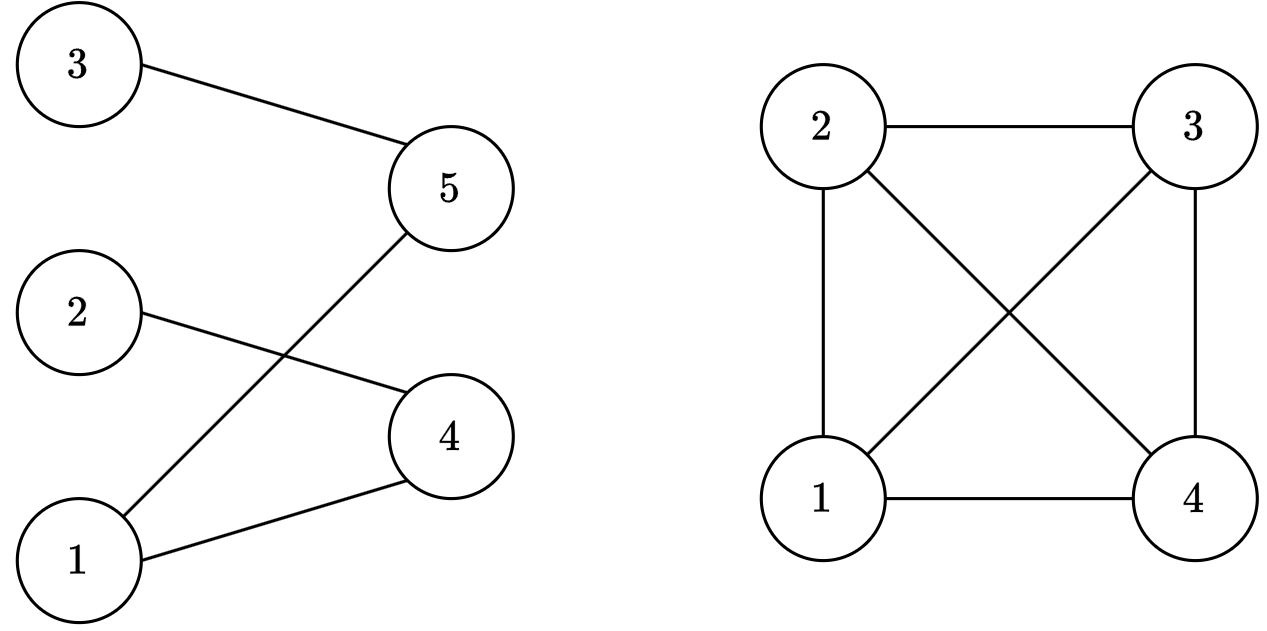
\includegraphics[width=0.5\linewidth]{images/bipcomp.png}
    \end{figure}
\end{example}
\begin{definition}[\textit{Outgoing cut}]
    Given a directed graph $G=(N,A)$ and $S \subset NM$, the \emph{outgoing cut} induced by $S$ is:
    \[ \delta^{+}(S)=\{(u,v) \in A \mid u \in S \land v \in N-S \} \]
\end{definition}
\begin{definition}[\textit{Incoming cut}]
    Given a directed graph $G=(N,A)$ and $S \subset NM$, the \emph{incoming cut} induced by $S$ is:
    \[ \delta^{-}(S)=\{(u,v) \in A \mid v \in S \land u \in N-S \} \]
\end{definition}
\begin{example}
    In the graph presented below, we can observe that:
    \begin{itemize}
        \item $\delta^{+}(\{1,4\})=\{(1,2),(4,2),(4,5)\}$
        \item $\delta^{-}(\{1,4\})=\{(3,4),(5,4)\}$
    \end{itemize}
    \begin{figure}[H]
        \centering
        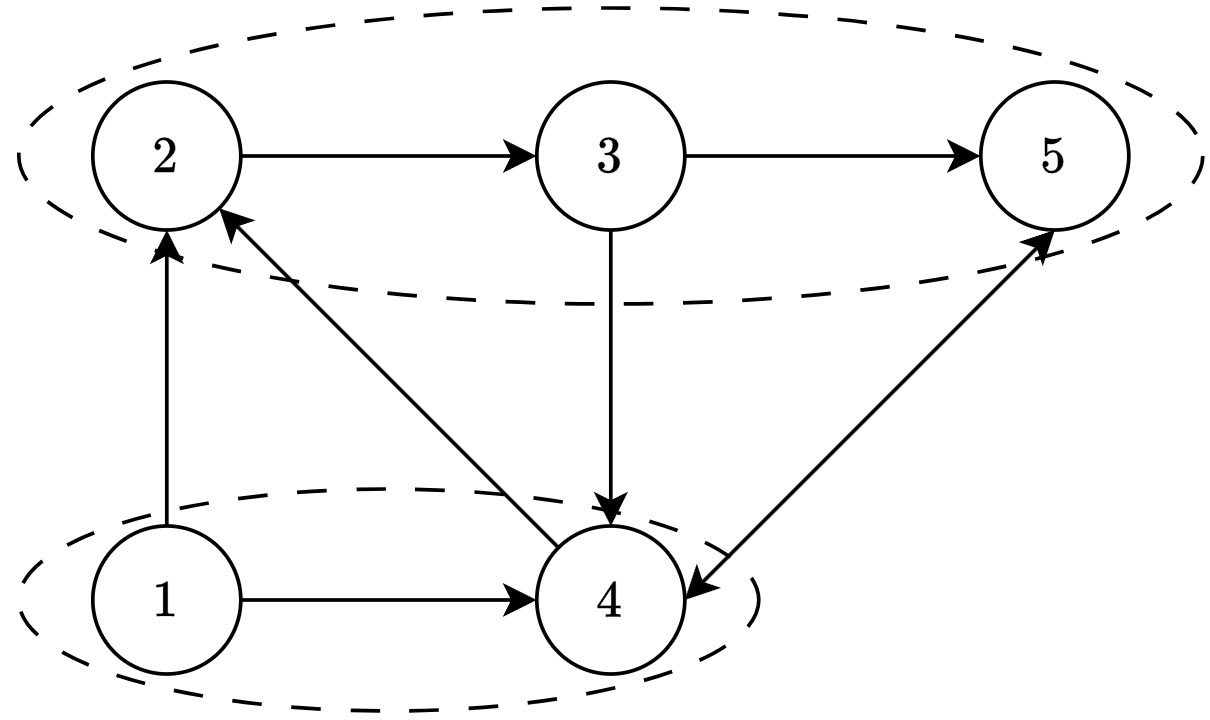
\includegraphics[width=0.4\linewidth]{images/cuts.png}
    \end{figure}
\end{example}
An undirected graph with $n$ nodes has at most $m=\dfrac{n(n-1)}{2}$ arcs. 
A directed graph with $n$ nodes has at most $m=n(n-1)$ arcs.
\begin{definition}[\textit{Dense graph}]
    For a given graph with $m$ representing the number of arcs or edges and $n$ representing the number of nodes, we classify a graph as dense when:
    \[m \approx n^2\]
\end{definition}
\begin{definition}[\textit{Sparse graph}]
    For a given graph with $m$ representing the number of arcs or edges and $n$ representing the number of nodes, we classify a graph as sparse when:
    \[m \ll n^2\]
\end{definition}

\paragraph*{Graph representation}
The most suitable method for representing a dense graph is by utilizing an $n \times n$ adjacency matrix, defined as follows:
\[
\begin{cases}
    a_{ij}=1 \:\:\:\:\:\: \text{if }(i,j) \in A \\
    a_{ij}=0 \:\:\:\:\:\: \text{otherwise}    
\end{cases}    
\]
Conversely, for a sparse graph, the most effective approach is to use lists of successors for each node.
\begin{example}
    The adjacency matrix for the depicted graph is as follows:
    \[A=\begin{bmatrix}
        0 & 1 & 0 & 1 & 0 \\
        0 & 0 & 1 & 0 & 0 \\
        0 & 0 & 0 & 1 & 1 \\
        0 & 1 & 0 & 0 & 1 \\
        0 & 0 & 0 & 1 & 0 
        \end{bmatrix}\]
    Furthermore, the list of successors is presented as follows:
    \[S(1)=\{2,4\} \:\:\: S(2)=\{3\} \:\:\:S(3)=\{4,5\} \:\:\: S(4)=\{2,5\} \:\:\: S(5)=\{4\} \:\:\:\]
    \begin{figure}[H]
        \centering
        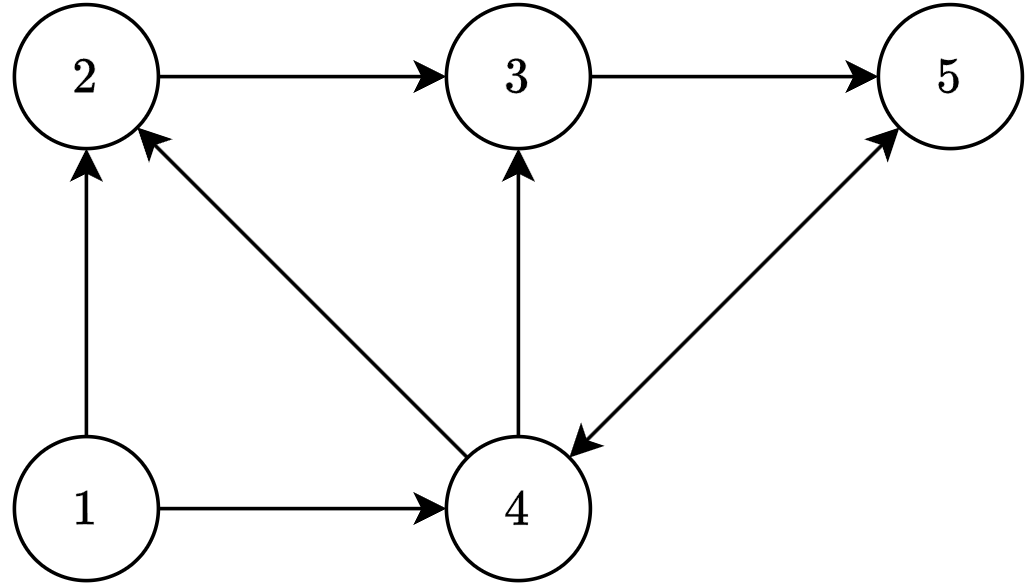
\includegraphics[width=0.3\linewidth]{images/graphs.png}
    \end{figure}
\end{example}
\begin{definition}[\textit{Sub-graph}]
    $G^{'}=(N^{'},E^{'})$ is a sub-graph of $G=(N,E)$ if $N^{'} \subseteq N$ and $E^{'} \subseteq E$. 
\end{definition}
\begin{definition}[\textit{Tree}]
    A tree $G_T=(N^{'},T)$ \emph{of $G$} is a connected and acyclic sub-graph of $G$. 
\end{definition}
\begin{definition}[\textit{Spanning tree}]
    $G_T=(N^{'},T)$ is a spanning tree of $G$ if it contains all nodes in $G$. 
\end{definition}
\begin{definition}[\textit{Leaves}]
    The leaves of a tree are the nodes of degree one. 
\end{definition}
\begin{example}
    Considering the provided graph:
    \begin{figure}[H]
        \centering
        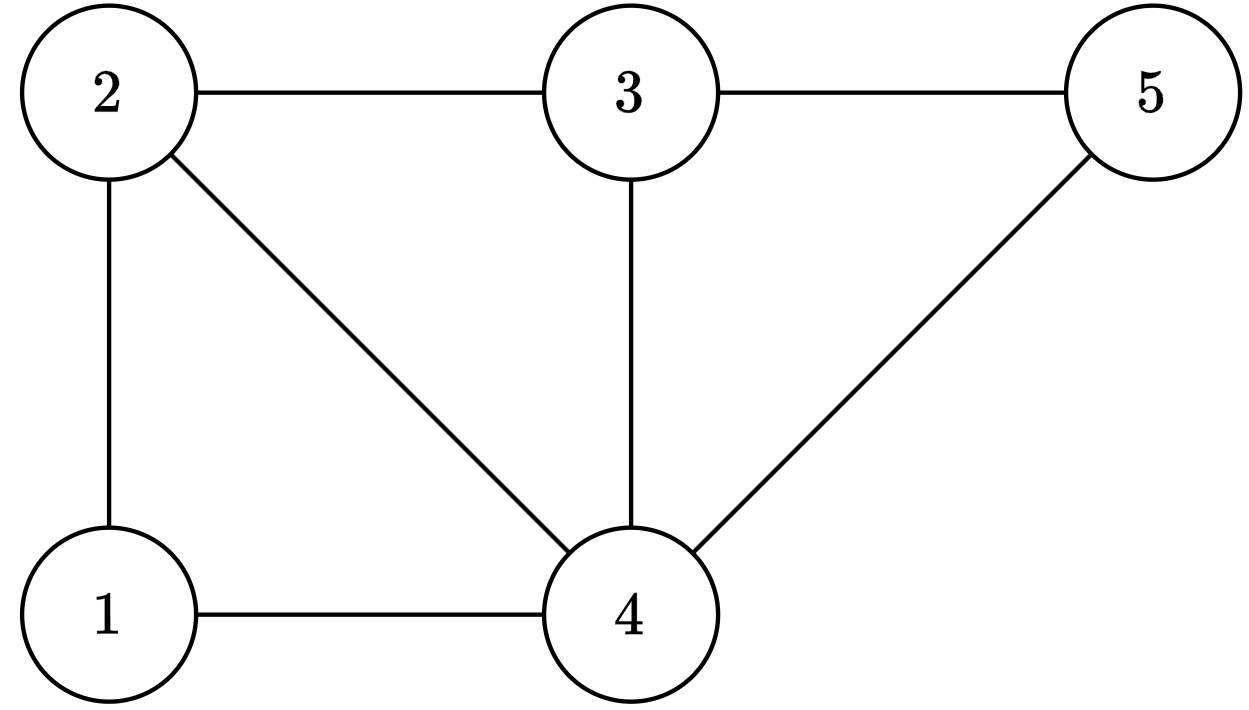
\includegraphics[width=0.3\linewidth]{images/sgraph.png}
    \end{figure}
    We can identify three different structures: a sub-graph, a tree, and a spanning tree. 
    These structures are visually depicted in the modified graph below:
    \begin{figure}[H]
        \centering
        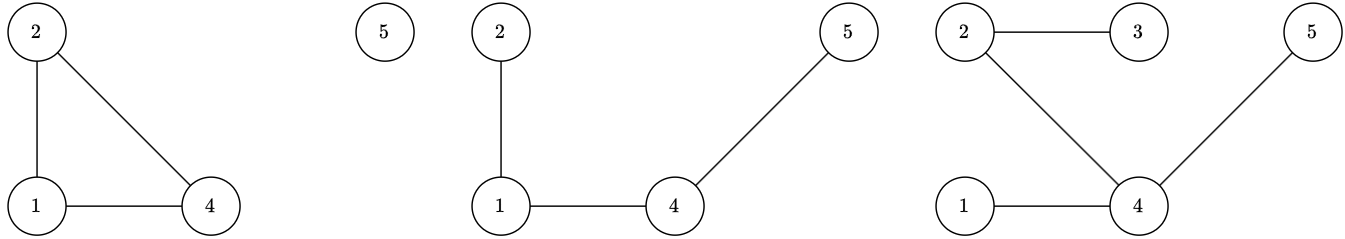
\includegraphics[width=0.8\linewidth]{images/sgraphmod.png}
    \end{figure}
\end{example}
\begin{property}
    Every tree with $n$ nodes has $n-1$ edges. 
\end{property}
\begin{proof}
    We will demonstrate this property with a proof by induction. 
    For the base case we have that the claim holds for $n=1$. 
    For the inductive step we have to show that, if this is true for trees with $n$ nodes, then it is also true for those with $n+1$ nodes. 
    Let $T_1$ be a tree with $n+1$ nodes and recall that any tree with $n \geq 2$ nodes has at least two leaves. 
    By deleting one of the leaf and its incident edge we obtain a tree $T_2$ with $n$ nodes. 
    By induction hypothesis, $T_2$ has $n-1$ edges. 
    Therefore, the tree $T_1$ has $n-1+1=n$ edges. 
\end{proof}
\begin{property}
    Any pair of nodes in a tree is connected via a unique path. 
\end{property}
\begin{property}
    By adding a new edge to a tree, we create a unique cycle. 
\end{property}
\begin{property}
    Let $G_T=(N,T)$ be a spanning tree of $G=(N,E)$. 
    Consider an edge $e \notin T$ and the unique cycle $C$ of $T \cup \{e\}$. 
    For each edge $f \in C-\{e\}$, the sub-graph $T\cup \{e\}-\{f\}$ is also a spanning tree of $G$. 
\end{property}